\documentclass[11pt]{article}

% ── Packages ──────────────────────────────────────────────────────────────
\usepackage[margin=1in]{geometry}
\usepackage{amsmath}
\usepackage{amssymb}
\usepackage{booktabs}
\usepackage{hyperref}
\usepackage{url}
\usepackage{microtype}
\usepackage{parskip}
\usepackage{setspace}
\usepackage{titlesec}
\usepackage{enumitem}
\usepackage{xcolor}
\usepackage{graphicx}
\usepackage{tikz}
\usetikzlibrary{shapes.geometric,arrows.meta,positioning,fit,backgrounds,calc}

\hypersetup{
  colorlinks=true,
  linkcolor=blue!70!black,
  citecolor=blue!70!black,
  urlcolor=blue!70!black
}

\titleformat{\section}{\large\bfseries}{\thesection}{1em}{}
\titleformat{\subsection}{\normalsize\bfseries}{\thesubsection}{1em}{}

\setlength{\parindent}{0pt}
\setlength{\parskip}{6pt}

% ── TikZ styles ───────────────────────────────────────────────────────────
\tikzset{
  pbox/.style 2 args={
    rectangle, rounded corners=4pt, draw=#1!70!black,
    fill=#1!10, text width=#2, minimum height=1.05cm,
    align=center, font=\small
  },
  gbox/.style={
    rectangle, rounded corners=4pt, draw=gray!55,
    fill=gray!7, text width=#1, minimum height=1.0cm,
    align=center, font=\small
  },
  outbox/.style={
    rectangle, rounded corners=4pt, draw=teal!60!black,
    fill=teal!8, text width=3.0cm, minimum height=0.9cm,
    align=center, font=\footnotesize
  },
  stobox/.style={
    rectangle, rounded corners=4pt, draw=orange!65!black,
    fill=orange!9, text width=11cm, minimum height=0.85cm,
    align=center, font=\small
  },
  mydiamond/.style={
    diamond, aspect=3.0, draw=blue!60!black,
    fill=blue!9, minimum width=4.0cm, minimum height=1.1cm,
    align=center, font=\small
  },
  arr/.style={-{Stealth[length=5pt]}, thick, gray!65!black},
  darr/.style={-{Stealth[length=5pt]}, thick, gray!65!black, dashed},
  lbl/.style={font=\footnotesize\itshape, text=gray!65!black}
}

% ── Title ─────────────────────────────────────────────────────────────────
\title{\textbf{CRUCIBLE: A Multi-Agent Framework for Automated\\
Annotation Rubric Calibration via Iterative\\
Inter-Judge Disagreement Resolution}}

\author{
  Bidit Das \\
  Independent Researcher \\
  Dallas, Texas, USA \\
  \texttt{biditdas18@gmail.com}
}

\date{June 2026}

% ══════════════════════════════════════════════════════════════════════════
\begin{document}
\maketitle

% ── Abstract ──────────────────────────────────────────────────────────────
\begin{abstract}
Annotation quality is a limiting factor in supervised learning pipelines
that rely on the LLM-as-judge paradigm. A domain-agnostic rubric applied to a
binary transcript classification task yielded only 53\% pairwise inter-judge
agreement---essentially at chance and
insufficient to produce reliable training labels. Manual rubric refinement
does not scale and introduces annotator-specific bias that usually goes unaudited and is hard to reproduce. We present \textbf{CRUCIBLE}, a multi-agent system that
automatically calibrates annotation rubrics through iterative disagreement
diagnosis and targeted revision. Three heterogeneous local judge models
independently evaluate a transcript corpus; a coordinator model (Claude Sonnet)
analyzes per-model criterion-level disagreement patterns and proposes rubric
revisions; the loop repeats until all domains converge or a fixed iteration budget is
exhausted, flagging any domain whose agreement stagnates. CRUCIBLE was developed to solve
a concrete annotation bottleneck in building a Signal-to-Noise Ratio (SNR)
classifier for YouTube educational content---the initial domain-agnostic rubric
drove inter-judge agreement no better than chance. Applied to 60 YouTube transcripts
across three content domains---General Education, Technology \& AI, and Career
\& Self-Improvement---CRUCIBLE reached 96.7\% and 81.7\%
weighted inter-judge agreement on two domains, while
the third domain failed to converge---its best rubric reaching only 70.0\%, near the
floor of the weighted metric---suggesting a model capability ceiling rather than a successful calibration.
Because raw agreement is inflated by label prevalence, we report chance-corrected
agreement (Fleiss' $\kappa$ and Gwet's AC1); these locate CRUCIBLE's value less in raising
raw agreement than in diagnosing whether residual disagreement is rubric-fixable,
capability-bounded, or prevalence-dominated.
The third
domain's stagnation revealed that one judge model systematically
misapplied a co-occurrence criterion that no rubric revision compensated for under this judge
and prompt setup. The system also detected and logged a degenerate judge (Gemma 2 9B, producing
identical LOW labels for all 60 transcripts), providing implicit quality
control. The calibrated rubrics, applied by a separate frontier ensemble (reported in the companion
paper), produced labels that trained a binary classifier on the SNR task achieving
F1\,=\,0.871 with recall\,=\,0.964 on the HIGH-signal class. Code and
calibration logs are available at
\url{https://github.com/biditdas18/rubric-calibration-agent}.
\end{abstract}

% ── 1. Introduction ───────────────────────────────────────────────────────
\section{Introduction}

The LLM-as-judge paradigm has become a standard component of annotation
pipelines in settings where human labeling is expensive, slow, or subject to
individual bias~\cite{zheng2023judging}. A single LLM prompted with an
evaluation rubric can produce labels at scale, but single-model annotation
carries systematic biases rooted in the model's training distribution,
instruction-following style, and boundary-case
interpretation~\cite{shi2024judging}. Multi-model ensembles reduce this risk,
but introduce a new dependency: the rubric must be precise enough that multiple
independent models reach consistent conclusions. A poorly specified rubric
produces disagreement not because the content is genuinely ambiguous, but
because different models resolve underspecified criteria differently.

This paper originates from a concrete failure of that kind. We were building a
Signal-to-Noise Ratio (SNR) framework\footnote{The SNR classifier is described
in a companion paper: Das, B.
(2026). Signal-to-Noise Ratio Detection in Educational Video Content: A
Binary Classification Framework Using Transcript Embeddings. SSRN.
\url{https://papers.ssrn.com/sol3/papers.cfm?abstract_id=6866745}. That
work cites CRUCIBLE as its annotation methodology.} for binary classification of YouTube educational video
transcripts---separating substantive instructional content (HIGH signal:
concrete actionable steps, methodological coherence, named frameworks) from
low-value filler (LOW signal: generic motivational advice, fear-based framing,
promotional material, repetition without progression). The task required
labeled training data reliable enough to train a lightweight classifier
deployable at inference scale.

The initial approach was a domain-agnostic rubric applied across a three-model
LLM ensemble. It yielded 53\% pairwise inter-judge agreement, close to the 50\% chance level for binary
pairwise agreement.
Two remedies were available: (1)~manually label a gold dataset per domain, or
(2)~automatically calibrate the rubrics until the ensemble converges.
Option~1 was rejected on two grounds. First, reviewing transcripts of 10--15
minute videos at the scale required is prohibitively time-intensive. Second,
and more fundamentally, manual annotation introduces annotator-specific bias that is reducible only through
multiple annotators and adjudication:
an annotator who values career development content intrinsically applies a
systematically different threshold than one who does not. Without a multi-annotator comparison, that bias goes unaudited and undisclosed---baked into every label silently.

We designed CRUCIBLE to solve this. It is a coordinator-mediated, iterative
calibration loop requiring no human reference labels and no domain expertise
beyond an initial rubric draft. Three heterogeneous local models serve as
judges; a frontier coordinator model diagnoses their disagreement patterns and
proposes targeted rubric revisions; the loop repeats until convergence or a fixed iteration budget is exhausted. The resulting domain-specific rubrics are versioned and auditable.
The labels they produce are silver quality---not gold---but empirically
validated against a measurable inter-judge criterion rather than a single
annotator's unchecked judgment.

The downstream result provides end-to-end evidence for the approach. The rubrics produced by CRUCIBLE were applied by a separate frontier ensemble (GPT-4o mini,
Gemini 2.5 Flash, Llama 3.3 70B; reported in the companion paper) to label the transcripts;
an SVM trained on those labels achieved F1\,=\,0.871 with recall\,=\,0.964 on the HIGH-signal
class, compared to a majority-class baseline of F1\,=\,0.000. We did not attempt training on the original 53\%-agreement
labels; the majority-class baseline (F1 = 0.000) indicates the task is non-trivial.

\textbf{The core contributions of this paper are:}

\begin{enumerate}[leftmargin=*, label=\arabic*.]

\item \textbf{An automated rubric calibration loop} with coordinator-mediated
disagreement diagnosis and targeted revision. Unlike prior rubric-generation and refinement systems, which are validated against
reference judgments or accuracy signals, CRUCIBLE studies a narrower setting: iterative
rubric revision driven solely by inter-judge disagreement, with no human reference labels at
any stage.

\item \textbf{The model capability ceiling finding.} The system empirically
distinguishes rubric-fixable disagreement (Technology \& AI: 76.7\%
$\rightarrow$ 81.7\% in one iteration) from model-capability-bounded disagreement
(Career \& Self-Improvement: failed to converge despite two revisions, with its best rubric at 70.0\%). This
distinction is not a failure; it is a diagnostic.

\item \textbf{Degenerate judge detection.} Gemma~2 9B produced LOW labels for all
60 transcripts---zero discriminative outputs. The system logged this
explicitly, enabling model replacement before calibration. This constitutes
implicit quality control on the judge panel.

\item \textbf{Per-domain convergence with regression checking.} Domains
converge independently; each iteration includes a regression check on
previously converged domains to detect rubric drift.

\item \textbf{Columnar evaluation order for local multi-model inference.}
Batching evaluation by model rather than by document reduces model-load events
from 180 to 3 total per iteration, cutting per-iteration runtime from $>$30
minutes (incomplete) to $\approx$17--20 minutes on consumer hardware.

\item \textbf{End-to-end consistency evidence.} The calibrated rubrics, applied downstream by a frontier ensemble, produced labels that
trained an SVM classifier achieving F1\,=\,0.871 and recall\,=\,0.964 on the
HIGH-signal class, consistent with rubric calibration quality translating to downstream classifier
performance.

\end{enumerate}

% ── 2. Related Work ───────────────────────────────────────────────────────
\section{Related Work}

\subsection{LLM-as-Judge}

The use of large language models as automated evaluators was formalized by
Zheng et al.~\cite{zheng2023judging} in the MT-Bench benchmark. Subsequent
work extended this paradigm to structured rubrics~\cite{liu2023geval},
fine-grained multi-dimensional scoring~\cite{kim2024prometheus}, and
customizable evaluation dimensions~\cite{fu2023gptscore}. A persistent finding is
that single-model judges exhibit systematic biases---position bias, verbosity
bias, and self-preference---that reduce
reliability~\cite{zheng2023judging, shi2024judging}. Multi-model ensembles have been proposed to
mitigate these biases~\cite{chan2023chateval}, but ensemble reliability still
depends on rubric quality.

\subsection{Rubric Design and Calibration}

LLM-Rubric~\cite{hashemi2024llmrubric} combines LLM predictions with a small
neural network to predict human judge annotations. AdaRubric~\cite{adarubric2026}
proposes task-adaptive rubric generation for agent evaluation.
Autorubric~\cite{autorubric2026} provides a unifying framework for rubric-based
evaluation across criterion types. None of these works addresses automated
iterative rubric \emph{revision}---they assume the rubric is fixed. Prior
rubric-refinement work that does iterate does so against human-labeled reference
data~\cite{patch2025rubric}. The system described here performs rubric revision
with no human input at any stage.
SciIF~\cite{sciif2026} pairs problems with a fixed catalog of scientific constraints and structured
verification rubrics, but treats the rubric as fixed rather than something to be revised.
Recent work also automates rubric generation and refinement: RRD~\cite{shen2026rrd} recursively
decomposes and filters rubric criteria, and GER-Eval~\cite{siro2026ger} has LLMs design and apply their
own rubrics. Both are still validated against reference judgments or accuracy signals; CRUCIBLE instead
drives revision purely from inter-judge agreement with no human reference labels.

\subsection{Disagreement Diagnosis}

Related self-deliberation mechanisms appear in evaluation frameworks such as
AraTable~\cite{aratable2025}, where a judge re-examines its own
assessment. Multi-agent debate~\cite{du2023improving} resolves disagreement through structured exchange
among models. These approaches are self-revision or debate; neither produces a generalized rubric revision that
improves agreement across the full corpus and on future evaluation runs.

\subsection{Multi-Agent Coordination}

Multi-agent debate frameworks~\cite{du2023improving} have been applied to
improve LLM output reliability through structured disagreement resolution.
CRUCIBLE applies the coordinator-mediator pattern asymmetrically: judge models
do not communicate with each other; only the coordinator sees aggregate
disagreement patterns and produces the revision.

\subsection{Annotation Bias and Scalability}

The annotation bottleneck has been addressed through weak
supervision~\cite{ratner2017snorkel}, programmatic
labeling~\cite{bach2019snorkel}, and knowledge distillation from frontier
models~\cite{hinton2015distilling}. CRUCIBLE is complementary: it produces
validated rubrics grounding ensemble annotation at any scale.

% ── 3. The CRUCIBLE System ────────────────────────────────────────────────
\section{The CRUCIBLE System}

\subsection{Problem Statement}

Given a corpus $\mathcal{D} = \{d_1, \ldots, d_N\}$ to be annotated with a
binary label $y \in \{H, L\}$, and an initial rubric $R^{(0)}$ specifying
criteria for each label, we seek a revised rubric $R^{(k)}$ such that the
weighted inter-judge agreement $A(R^{(k)}, \mathcal{D}) \geq \tau$ for a
target threshold $\tau$, with the revision process requiring no human-labeled
reference data.

The key insight is that inter-judge disagreement encodes rubric
underspecification: when two competent models applying the same rubric reach
opposite conclusions on the same document, the rubric has not resolved the
case. A coordinator with visibility into both decisions and the criterion-level
justifications can identify \emph{which criterion was misapplied and
how}---and propose a targeted revision to close the gap.

\subsection{Architecture}

Figure~\ref{fig:arch} illustrates the full system. Judge models operate
independently and in isolation from each other; only the coordinator sees their
combined outputs. The rubric revision loop is the only feedback path---there
is no human in the loop after initialization.

\begin{figure}[ht]
\centering
\resizebox{\textwidth}{!}{%
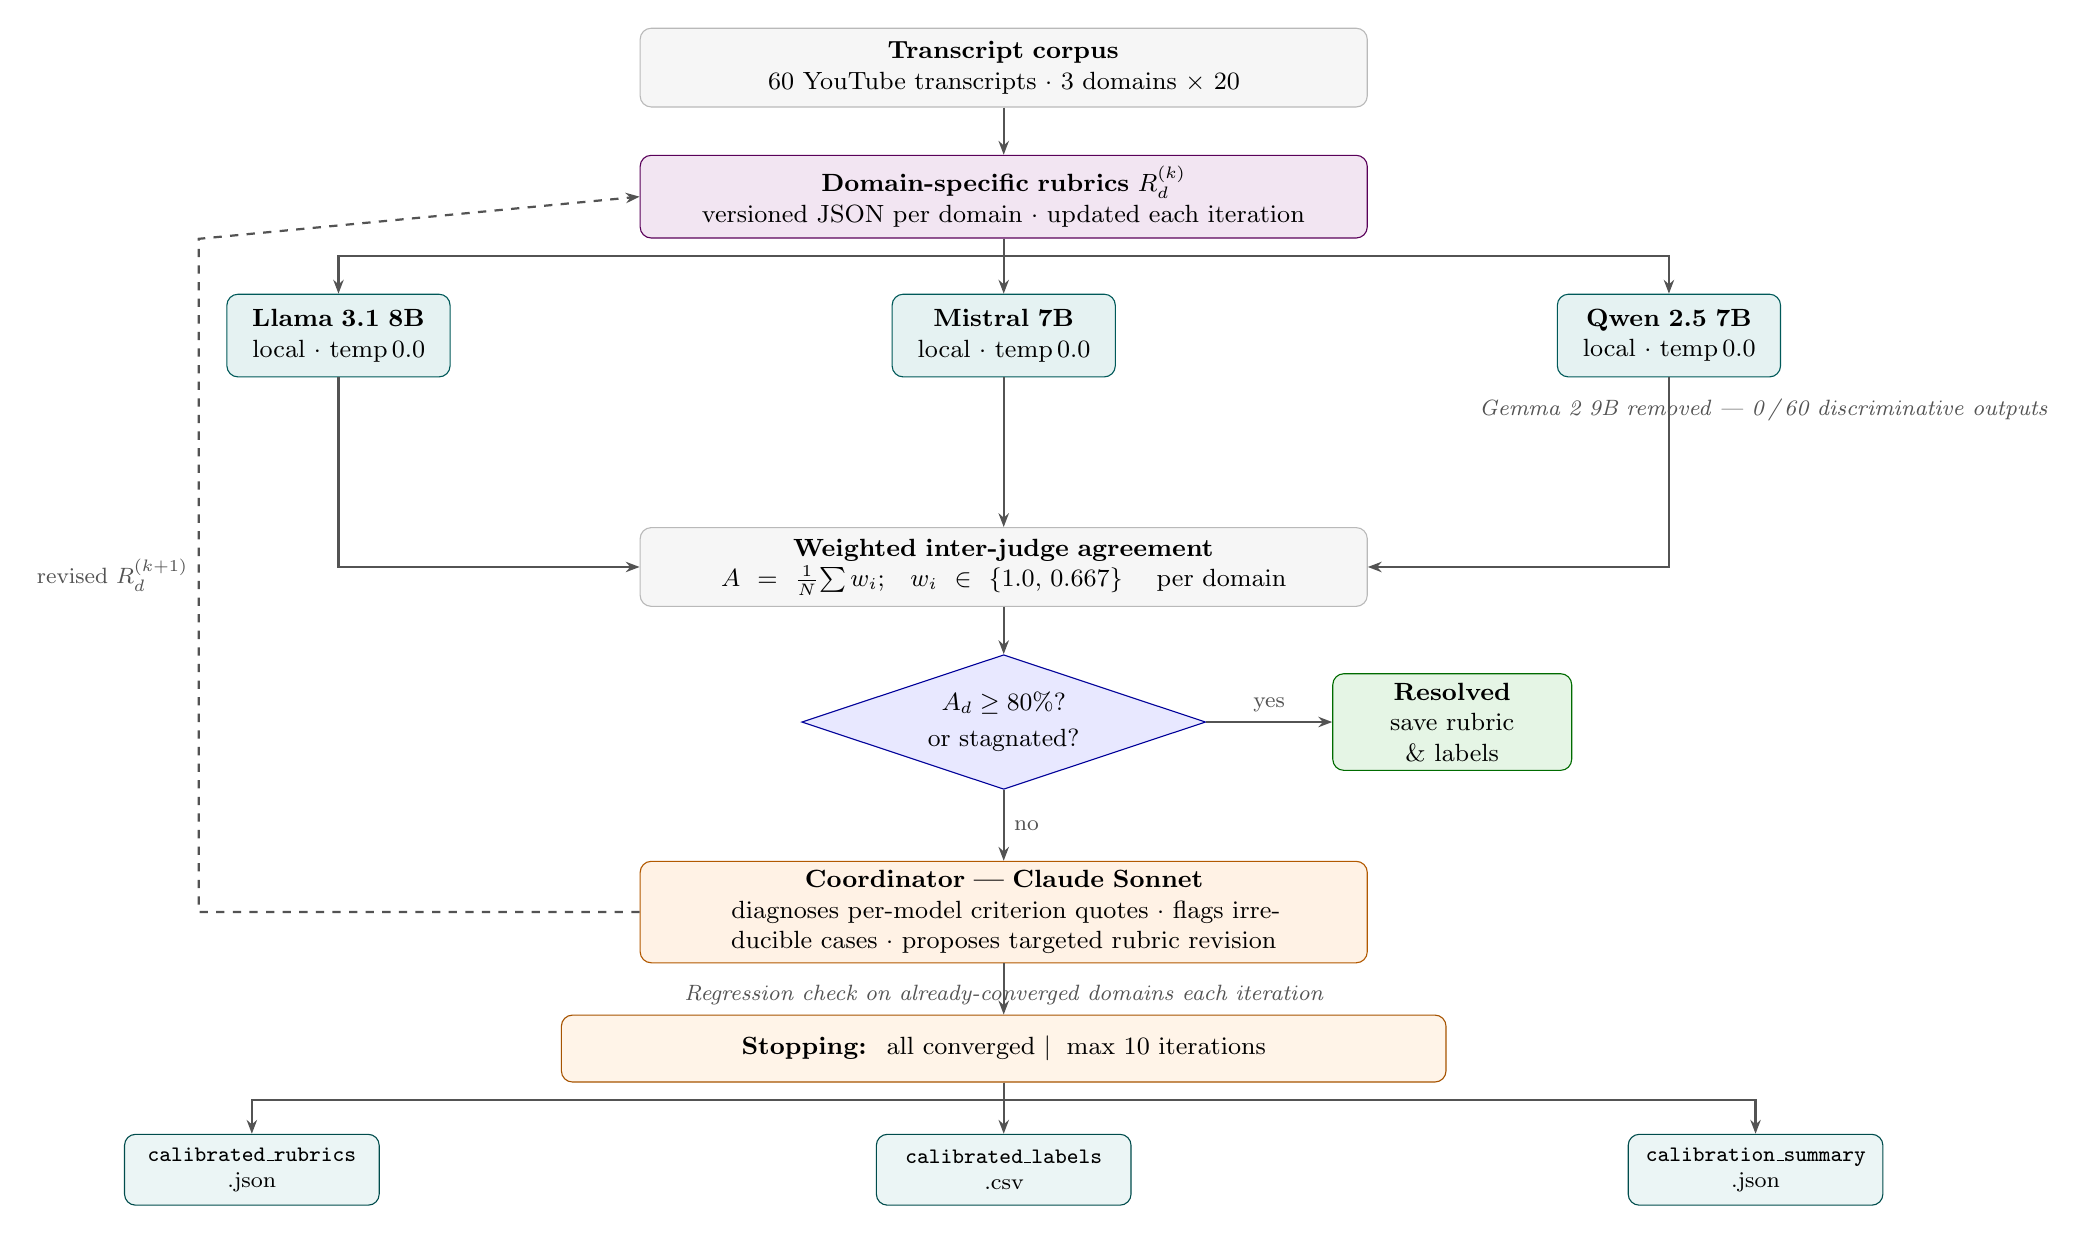
\begin{tikzpicture}[node distance=0.6cm and 0.5cm]

% Input
\node[gbox=9.0cm] (corpus)
  {\textbf{Transcript corpus}\\
   60 YouTube transcripts $\cdot$ 3 domains $\times$ 20};

% Rubrics
\node[pbox={violet}{9.0cm}, below=of corpus] (rubrics)
  {\textbf{Domain-specific rubrics} $R_d^{(k)}$\\
   versioned JSON per domain $\cdot$ updated each iteration};

% Judges
\node[pbox={teal}{2.6cm}, below left=0.7cm and 2.4cm of rubrics] (llama)
  {\textbf{Llama 3.1 8B}\\local $\cdot$ temp\,0.0};

\node[pbox={teal}{2.6cm}, below=0.7cm of rubrics] (mistral)
  {\textbf{Mistral 7B}\\local $\cdot$ temp\,0.0};

\node[pbox={teal}{2.6cm}, below right=0.7cm and 2.4cm of rubrics] (qwen)
  {\textbf{Qwen 2.5 7B}\\local $\cdot$ temp\,0.0};

\node[lbl, below=0.15cm of qwen, xshift=1.2cm]
  {Gemma 2 9B removed --- 0\,/\,60 discriminative outputs};

% Agreement
\node[gbox=9.0cm, below=1.9cm of mistral] (agree)
  {\textbf{Weighted inter-judge agreement}\\
   $A = \tfrac{1}{N}\!\sum w_i$;\quad
   $w_i \in \{1.0,\,0.667\}$ \quad per domain};

% Decision diamond
\node[mydiamond, below=0.6cm of agree] (dec)
  {$A_d \geq 80\%$?\\[2pt]or stagnated?};

% Converged
\node[pbox={green!60!black}{2.8cm}, right=1.6cm of dec] (conv)
  {\textbf{Resolved}\\save rubric \& labels};

% Coordinator
\node[pbox={orange}{9.0cm}, below=0.9cm of dec] (coord)
  {\textbf{Coordinator --- Claude Sonnet}\\
   diagnoses per-model criterion quotes $\cdot$
   flags irreducible cases $\cdot$
   proposes targeted rubric revision};

\node[lbl, below=0.15cm of coord]
  {Regression check on already-converged domains each iteration};

% Stopping
\node[stobox, below=0.65cm of coord] (stop)
  {\textbf{Stopping:}\;
   all converged \textbar\;
   max 10 iterations};

% Outputs
\node[outbox, below left=0.65cm and 2.3cm of stop] (o1)
  {\texttt{calibrated\_rubrics}\\.json};
\node[outbox, below=0.65cm of stop] (o2)
  {\texttt{calibrated\_labels}\\.csv};
\node[outbox, below right=0.65cm and 2.3cm of stop] (o3)
  {\texttt{calibration\_summary}\\.json};

% ── Arrows ──────────────────────────────────────────────────────────────
\draw[arr] (corpus) -- (rubrics);
\draw[arr] (rubrics.south) -- ++(0,-0.22) -| (llama.north);
\draw[arr] (rubrics.south) -- (mistral.north);
\draw[arr] (rubrics.south) -- ++(0,-0.22) -| (qwen.north);

\draw[arr] (llama.south) -- ++(0,-0.22) |- (agree.west);
\draw[arr] (mistral.south) -- (agree.north);
\draw[arr] (qwen.south)  -- ++(0,-0.22) |- (agree.east);

\draw[arr] (agree) -- (dec);
\draw[arr] (dec.east) -- node[above,font=\footnotesize]{yes} (conv.west);
\draw[arr] (dec.south) -- node[right,font=\footnotesize]{no} (coord.north);

% Feedback loop: coordinator back to rubrics
\draw[darr] (coord.west) -- ++(-5.6,0)
  -- node[left,font=\footnotesize]{revised $R_d^{(k+1)}$}
     ++(0, 8.55)
  -- (rubrics.west);

\draw[arr] (coord.south) -- (stop.north);

\draw[arr] (stop.south) -- ++(0,-0.22) -| (o1.north);
\draw[arr] (stop.south) -- (o2.north);
\draw[arr] (stop.south) -- ++(0,-0.22) -| (o3.north);

\end{tikzpicture}
}
\caption{CRUCIBLE system architecture. Judge models operate independently
at temperature~0.0. The dashed arrow is the only feedback path: revised rubrics
flow back into the next iteration. No human input occurs after initialization.}
\label{fig:arch}
\end{figure}

\subsection{System Components}

\textbf{Judge models.} Three heterogeneous local models running at
temperature~0.0 via Ollama: Llama~3.1~8B (Meta), Mistral~7B (Mistral AI), and
Qwen~2.5~7B (Alibaba). Temperature~0.0 yields near-deterministic outputs, isolating
rubric quality as the variable of interest. The three models were chosen to
represent different training lineages, maximizing the diagnostic value of their
disagreements.
These local models serve as the calibration instrument only; production labeling in the
downstream application uses a separate, stronger frontier ensemble (companion paper).

\textbf{Coordinator model.} Claude Sonnet (claude-sonnet-4-6), via API. The
coordinator receives: (a)~the current rubric, (b)~per-model label assignments
and criterion-level justification quotes for each disagreement case, and
(c)~disagreement counts per criterion. It produces a structured JSON revision
proposal specifying which criterion to modify and the revised text.

\textbf{Agreement metric.}
\begin{equation}
  A = \frac{1}{N} \sum_{i=1}^{N} w_i, \qquad
  w_i = \begin{cases}
    1.0   & \text{all three judges agree} \\
    0.667 & \text{exactly two judges agree}
  \end{cases}
\end{equation}
For three judges on a binary label, every item is either unanimous ($w=1.0$) or a
two--one majority ($w=0.667$); the no-majority case cannot occur, so $A$ is bounded below
by $0.667$. Under independent judges the expected value of $A$ is approximately $0.75$,
which should be read as the chance level for this metric; label skew can raise it further.

All-agree rate (unanimous three-way agreement) is tracked separately as a
stricter secondary metric.

\subsection{Calibration Loop}

\textbf{Initialization.} Domain-specific rubrics $R_d^{(0)}$ are written at
moderate abstraction---sufficient to convey intent but not yet precise enough
to resolve edge cases consistently.

\textbf{Iteration $k$:}
\begin{enumerate}[leftmargin=*, noitemsep]
  \item All three judges evaluate all documents using $\{R_d^{(k)}\}$.
  \item Weighted agreement $A_d^{(k)}$ is computed per domain.
  \item For each non-converged, non-stagnated domain with $A_d^{(k)} < \tau$:
    \begin{enumerate}[label=\alph*., noitemsep]
      \item Extract disagreement cases (at least one judge diverged).
      \item Assemble per-model criterion quotes for each case.
      \item Coordinator diagnoses and proposes revision.
      \item If valid JSON: $R_d^{(k+1)} \leftarrow \mathrm{revise}(R_d^{(k)})$.
      \item Irreducible cases (genuine ambiguity, not rubric failure) are logged
            and excluded from stagnation counting.
    \end{enumerate}
  \item Regression check on each already-converged domain.
\end{enumerate}

\textbf{Stopping.} A domain is marked \emph{stagnated} when $\Delta A_d \leq 0$ for three
consecutive iterations; it is then excluded from further revision and held at its current
rubric, but this does not terminate the loop. The loop terminates only when (a)~all domains
have converged or (b)~the maximum of 10 iterations is reached. Because Career \&
Self-Improvement never converged, the present run continued to the 10-iteration cap, with
converged domains monitored by regression checks and the stagnated domain held in place.

\subsection{Judge Quality Control}

Prior to the primary run, each candidate judge is evaluated for discriminative
validity. A degenerate judge---one assigning a single label to all
documents---provides zero inter-judge signal and pollutes agreement scores.

During development, Gemma~2 9B produced LOW labels for all 60 transcripts
across all domains (0\% HIGH rate). This is consistent with treating LOW
criteria as a checklist to confirm rather than a comparative threshold to apply.
Gemma~2 9B was replaced with Qwen~2.5~7B before the calibration run reported here.

\subsection{Columnar Evaluation Order: An Engineering Optimization}

The order in which judge models are invoked across the corpus has a dramatic
effect on runtime. The naive \emph{row-wise} approach:
\[
  T_1 \to [\text{Llama, Mistral, Qwen}] \to
  T_2 \to [\text{Llama, Mistral, Qwen}] \to \cdots
\]
requires Ollama to load, run, and unload three model weight sets for every
transcript. On consumer hardware with limited VRAM, each model switch incurs a
cold-load penalty. Across 60 transcripts and 3 models per transcript, this
produces 180 model-load events per iteration. In practice, this scheme could
not complete a single iteration within 30 minutes and was cancelled.

The fix draws on a principle from columnar database design: group operations by
column (model) rather than by row (transcript):
\[
  \underbrace{\text{Llama} \to 60\text{ transcripts}}_{\text{col.\,1}}
  \;\to\;
  \underbrace{\text{Mistral} \to 60\text{ transcripts}}_{\text{col.\,2}}
  \;\to\;
  \underbrace{\text{Qwen} \to 60\text{ transcripts}}_{\text{col.\,3}}
\]
This reduces model-load events from 180 to 3 total per iteration. Each model
loads once and remains resident in memory for its full 60-transcript pass.
Result: each iteration completed in 17--20 minutes on a consumer MacBook with
no GPU, making a 10-iteration calibration run (170.7 minutes total; the run terminated
at the maximum-iteration cap of 10 iterations) fully tractable.

% ── 4. Experimental Setup ─────────────────────────────────────────────────
\section{Experimental Setup}

\textbf{Task and corpus.} The target task is binary classification of YouTube
educational video transcripts under the SNR taxonomy: HIGH signal (substantive
instructional content: concrete actionable steps, methodological coherence,
named frameworks) vs.\ LOW signal (generic motivational advice, fear-based
framing, promotional material, repetition without progression). The corpus
comprises 60 transcripts across three domains (20 per domain): General
Education, Technology \& AI, and Career \& Self-Improvement. Transcripts
represent 10--15 minute videos in English.

\textbf{Initial rubrics.} Three domain-specific rubrics at version~0, each
specifying HIGH-signal criteria (methodological coherence, specificity,
informational novelty, solution orientation) and LOW-signal patterns (generic
advice, repetition, fear-based framing, promotional content, logical fallacies)
with domain-appropriate threshold language.

\textbf{Target threshold.} $\tau = 0.80$.

\textbf{Coordinator retry.} Up to 3 retries per call on JSON parsing failure;
5-second delay between attempts.

\textbf{Runtime.} 17--20 minutes per iteration (columnar order). 170.7 minutes
total; the run terminated at the maximum-iteration cap of 10 iterations. Consumer MacBook, no GPU.

\textbf{Baseline.} Domain-agnostic rubric: 53\% pairwise agreement.

% ── 5. Results ────────────────────────────────────────────────────────────
\section{Results}
\label{sec:results}

\subsection{Per-Domain Convergence}

\begin{table}[ht]
\centering
\caption{Calibration results per domain.}
\label{tab:results}
\small
\begin{tabular}{lccccccl}
\toprule
\textbf{Domain} &
\textbf{Initial $A$} &
\textbf{Best $A$} &
\textbf{All-agree} &
\textbf{Fleiss $\kappa$} &
\textbf{Gwet AC1} &
\textbf{Rubric ver.} &
\textbf{Status} \\
\midrule
General Education    & 96.7\% & 96.7\% & 90.0\% & $-0.034$ & $+0.929$ & v0 (0 changes) & Converged, iter.\,1 \\
Technology \& AI     & 76.7\% & 81.7\% & 45.0\% & $+0.246$  & $+0.286$ & v1 (1 change)  & Converged, iter.\,2 \\
Career \& Self-Impr. & 68.4\% & 70.0\% & 10.0\% & $-0.350$  & $-0.080$ & v1 (best of 2) & Stagnated \\
\bottomrule
\end{tabular}
\end{table}

General Education converged immediately in iteration~1 with no rubric revision.
Educational content with clear structural markers (lecture format, sequential
explanation, named frameworks) produced consistent judgments across all models.

Technology \& AI required one revision. The coordinator diagnosed that
Qwen~2.5~7B was reading HIGH criterion~1 too narrowly---requiring
production-system experience where the rubric intended methodological grounding.
The revised criterion made the threshold explicit; agreement rose from 76.7\%
to 81.7\%, crossing the 80\% target in one step.

Career \& Self-Improvement required two revision attempts: the first (v1) reached the best
agreement of 70.0\%, the second (v2) regressed to 68.4\% and was discarded, so v1 was retained.
Agreement never approached the 80\% target.
The coordinator's diagnosis across iterations~1 and~2 consistently identified the
same failure: Qwen~2.5~7B applied LOW criterion~1 (generic motivational
language) to any transcript containing motivational phrasing, regardless of
whether procedural content co-occurred. Revisions made the co-occurrence
condition progressively more explicit, but the model continued misapplying the
criterion. The coordinator flagged this as a model capability ceiling: the
model was failing to apply the co-occurrence condition consistently across long transcripts---a limitation at the model level, not a rubric
ambiguity.

We report Fleiss' $\kappa$ and Gwet's AC1 alongside raw weighted agreement, because raw
agreement is inflated by label prevalence. The three domains separate cleanly under
chance correction. Technology \& AI shows fair agreement ($\kappa = +0.25$, AC1 = $+0.286$)---the
only domain where a rubric revision carried agreement to the convergence target. Career \&
Self-Improvement shows below-chance agreement ($\kappa = -0.35$, AC1 = $-0.080$): the
judges are systematically anti-correlated, the quantitative signature of the capability
ceiling, since no rubric revision can raise agreement when one judge applies a criterion
inconsistently with the other two. General Education shows $\kappa \approx 0$ despite 96.7\%
raw agreement; this is the known prevalence paradox of $\kappa$ under skewed marginals~\cite{gwet2008} (the
domain is roughly 97\% one class), and Gwet's AC1 = $+0.929$, which is robust to
prevalence, indicates the agreement is genuine rather than chance-driven. The practical point
is that CRUCIBLE's contribution is not raising raw agreement per se---raw agreement is
base-rate-dependent---but diagnosing which regime a domain occupies: rubric-fixable,
capability-bounded, or prevalence-dominated.

\textbf{Initialization vs.\ iteration.} We separate how much of the
improvement over the 53\% domain-agnostic baseline is attributable to
writing a domain-specific starting rubric versus the iterative revision
loop itself. In General Education, initialization alone (iteration~1)
achieved 96.7\%---identical to the final result; the revision loop
contributed nothing because none was needed. In Technology \& AI,
initialization brought agreement from 53\% to 76.7\% ($\approx$83\% of the
total 28.7-point gain), and one revision then added the remaining 5.0
points needed to cross threshold. In Career \& Self-Improvement,
initialization brought agreement from 53\% to 68.4\% ($\approx$91\% of the
17.0-point gain observed at best); one revision (v1) added a further 1.6
points before a second revision (v2) regressed performance and was
discarded. Across all three domains, domain-specific initialization
accounts for the substantial majority of total improvement (83--100\%,
depending on domain); the iterative loop's contribution is smaller in
absolute terms, necessary to cross threshold in Technology \& AI, and
attempted-but-unhelpful in Career \& Self-Improvement---itself informative,
as it is what let us distinguish a rubric-fixable domain from one exhibiting
the capability-ceiling pattern investigated further in
Section~\ref{sec:cotresults}.

\subsection{Convergence Trajectory}

\begin{table}[ht]
\centering
\caption{Weighted agreement (\%) per domain across iterations.
\checkmark\,=\,converged; $\triangle$\,=\,no improvement over best. Career's second revision (v2) regressed at iteration~3 and was not retained;
iterations~4--10 show no further improvement. The retained output is the best rubric, v1
(70.0\%, iteration~2).}
\label{tab:trajectory}
\small
\begin{tabular}{cccc}
\toprule
\textbf{Iter.} & \textbf{Career \& SI} & \textbf{Tech \& AI} & \textbf{Gen.\ Edu.} \\
\midrule
1    & 68.4              & 76.7              & 96.7\,\checkmark \\
2    & 70.0              & 81.7\,\checkmark  & 96.7\,\checkmark \\
3    & 68.4\,$\triangle$ & 81.7\,\checkmark  & 96.7\,\checkmark \\
4--10 & 68.4\,$\triangle$ & 81.7\,\checkmark  & 96.7\,\checkmark \\
\bottomrule
\end{tabular}
\end{table}

Both converged domains remained stable across all subsequent iterations;
regression checks confirmed no drift.
For Career \& Self-Improvement, the second revision (v2) regressed to 68.4\% at
iteration~3 and was rejected; no later revision exceeded the best observed rubric, so the
retained system output is v1 at 70.0\% from iteration~2. Agreement never reached the 80\% target.

\subsection{Downstream Validation: SNR Classifier Performance}

The calibrated rubrics were used to drive labeling for a lightweight SVM classifier on the
SNR binary classification task. Real transcripts labeled using CRUCIBLE-calibrated rubrics (applied by a separate frontier
ensemble, per the companion paper) were combined with 300 synthetically generated transcripts
for class balance, and the classifier was evaluated on a held-out set of 60 real transcripts.

\begin{center}
\small
\begin{tabular}{lcc}
\toprule
\textbf{Model} & \textbf{F1 (HIGH signal)} & \textbf{Recall (HIGH signal)} \\
\midrule
SVM on rubric-calibrated labels & 0.871 & 0.964 \\
Majority-class baseline  & 0.000 & ---   \\
\bottomrule
\end{tabular}
\end{center}

We did not train a classifier on the original 53\%-agreement labels; the majority-class
baseline (F1 = 0.000) indicates the task is non-trivial, and the F1 = 0.871 result reflects
the gain from labels produced with the calibrated rubrics.
The improvement is attributable to two factors working jointly: domain-specific rubric
calibration, which produced the rubrics the frontier ensemble applied, and the ensemble
labeling methodology, which makes residual model-level bias legible and diagnosable rather
than invisible. The classifier performance serves as
end-to-end consistency evidence for the calibrated rubrics: a frontier ensemble applying
them produced labels that train a strong classifier. Because the held-out labels were produced by the same silver-labeling methodology rather
than independent human gold labels, this F1 reflects internal consistency with the labeling
pipeline rather than external, human-validated accuracy. Full experimental
details of the SNR classifier---dataset construction, synthetic augmentation
strategy, and complete evaluation protocol---will be reported in the companion
paper currently in preparation (see footnote~1).

\textbf{Train/test split and label independence.} The classifier is trained
on 389 transcripts: 89 real transcripts with silver labels assigned via the
same calibrated-rubric ensemble methodology, combined with 300 synthetic
transcripts (150 HIGH, 150 LOW, balanced across domains) generated from
structured prompts with labels correct by construction. Evaluation uses a
disjoint, held-out set of 60 real transcripts---the same 60-transcript
corpus used throughout this paper---selected and labeled prior to any
classifier training. The 89 training-supplement transcripts and 300
synthetic transcripts are disjoint from the evaluation set by construction:
the training supplement was drawn from channels not represented in the
evaluation set, and synthetic transcripts correspond to no real video. We
note directly, per the concern motivating Section~\ref{sec:humanval}, that
the evaluation labels are \emph{not} independent of the calibration process
in the sense of external ground truth---they are assigned by the same class
of frontier-ensemble judges used for the training supplement, applying the
calibrated rubric. This is precisely the circularity Section~\ref{sec:humanval}
is designed to address: human consensus and calibrated-panel labels agree
at 90\% (General Education), 50\% (Technology \& AI), and 50\% (Career \&
Self-Improvement)---figures that should be read alongside, and as a caveat
on, the F1 reported above. The F1 score demonstrates the calibrated labels
are \emph{learnable} by a downstream classifier; it does not by itself
demonstrate the labels are \emph{correct}.

\subsection{Irreducible Cases}

The coordinator flagged Technology \& AI transcripts 6 and~7 as
irreducible---genuine content ambiguity rather than rubric failures.
Transcript~6 mixed procedural and motivational content; Transcript~7 presented
AI ethics discussion with strong conceptual rigor but no clear actionable steps.
Both were excluded from stagnation counting.

\subsection{Human Validation}
\label{sec:humanval}

All three reviewers of an earlier version of this work raised the same
concern: inter-judge agreement among LLM annotators may reflect shared
model bias rather than label correctness, and without a human reference
point, convergence cannot be distinguished from consensus error. We
address this directly with an independent human validation study.

\subsubsection{Design}

We recruited three independent annotators per domain (nine total) via
Prolific~\cite{palan2018prolific}, stratified by domain (10 transcripts per
domain, sampled from the 60-transcript corpus, plus one hidden
attention-check item per domain not included in the analysis below).
Annotators were shown only the raw transcript text---not the calibrated
rubric, not the domain label, and not CRUCIBLE's output---and asked to
judge, in their own words, whether each transcript was substantive and
valuable or generic and low-value, with a mandatory written justification.
This open-judgment design is deliberate: showing annotators the calibrated
rubric would test whether humans can \emph{follow} CRUCIBLE's criteria, not
whether CRUCIBLE's criteria independently match human judgment. Quality was
enforced via a hidden attention-check item per domain (adversarial or
unambiguous content with a known expected label), a mandatory
content-grounded justification, and post-hoc rejection of submissions that
failed the attention check or gave non-evaluative responses (one submission
was rejected on this basis and replaced).

\subsubsection{Results}

We report two quantities per domain: (1)~inter-annotator agreement among
the three humans, via Fleiss' $\kappa$ and Gwet's AC1~\cite{gwet2008}, and
(2)~the agreement between human majority-vote consensus and CRUCIBLE's
calibrated label for the same transcript, with 95\% bootstrap confidence
intervals (10{,}000 resamples) given the small per-domain sample.

\begin{table}[ht]
\centering
\caption{Human validation results per domain. Human $\kappa$/AC1 measure
agreement among the three annotators; Human vs.\ CRUCIBLE reports the
percentage of transcripts where human majority-vote consensus matches
CRUCIBLE's calibrated label, with 95\% bootstrap CI.}
\label{tab:humanval}
\small
\begin{tabular}{lcccc}
\toprule
\textbf{Domain} & \textbf{Human $\kappa$} & \textbf{Human AC1} &
\textbf{Human vs.\ CRUCIBLE} & \textbf{95\% CI} \\
\midrule
General Education         & 0.04 & 0.63 & 90.0\% & [70.0\%, 100.0\%] \\
Technology \& AI          & 0.04 & 0.63 & 50.0\% & [20.0\%, 80.0\%]  \\
Career \& Self-Impr.      & 0.33 & 0.33 & 50.0\% & [20.0\%, 80.0\%]  \\
\midrule
\textbf{Overall}          & ---  & ---  & \textbf{63.3\%} & \textbf{[46.7\%, 80.0\%]} \\
\bottomrule
\end{tabular}
\end{table}

General Education and Technology \& AI show identical $\kappa$/AC1 by
coincidence of vote-count distribution shape across their 10 items, verified
directly against the raw annotation tables, not a computation error.

The confidence intervals for Technology \& AI and Career \& Self-Improvement
overlap substantially, and both differ from General Education's interval
only at the boundary; we report the domain-level distinction below as
supported by the \emph{pattern} across human-human and human-model agreement
jointly, not by the point estimates in isolation, which alone are not
statistically distinguishable at this sample size.

These results support three distinct conclusions, one per domain:

\textbf{General Education: validated.} Human annotators agree with each
other at a moderate-to-good level (AC1\,=\,0.63) and agree with CRUCIBLE's
label 90\% of the time. This is consistent with this domain's fast, stable
convergence during calibration (Table~\ref{tab:results}: 96.7\% agreement,
v0 rubric, no revisions) and provides direct evidence that convergence here
reflects genuine label validity, not shared model artifact.

\textbf{Technology \& AI: a genuine model failure, not domain ambiguity.}
Human annotators agree with each other at the same rate as General
Education (AC1\,=\,0.63)---the task itself is well-posed and humans can
perform it consistently. Yet human consensus matches CRUCIBLE's label only
50\% of the time. Because human-human agreement is high while
human-CRUCIBLE agreement is low, this is not a case of an inherently
ambiguous domain; it is direct evidence that CRUCIBLE's confident
convergence (81.7\% inter-judge agreement, crossing our calibration
threshold) \emph{masked} a systematic divergence from human judgment. This
is precisely the failure mode reviewers warned against: high automated
agreement gave no signal that this domain's labels were less reliable than
General Education's, despite the two domains being empirically
indistinguishable by agreement metrics alone.

\textbf{Career \& Self-Improvement: domain ambiguity, not (only) model
failure.} Human annotators themselves show markedly lower agreement
(AC1\,=\,0.33) than in the other two domains. Since humans cannot
consistently agree with each other on this domain, CRUCIBLE's own
stagnation here (Table~\ref{tab:results}: 68.4\%--70.0\%, never crossing
threshold) is at least partly attributable to genuine task difficulty
rather than model failure alone. This nuances---without fully
resolving---our capability-ceiling diagnosis (Section~\ref{sec:cotresults}
tests this directly): the ceiling may be substantially a property of the
content itself, not solely the judge models.

\subsubsection{Implications}

These results require us to revise the framing of CRUCIBLE's central claim.
Automated inter-judge convergence is \emph{necessary but not sufficient}
evidence of label quality: it correctly identified General Education as
reliable and correctly flagged Career \& Self-Improvement as difficult, but
it failed to distinguish Technology \& AI's unreliable convergence from
General Education's valid convergence, despite near-identical agreement
statistics. We therefore do not claim CRUCIBLE eliminates the need for
human oversight; we show instead that periodic, targeted human
validation---at the scale used here, a small stratified sample per
domain---is necessary to determine \emph{which} domains' automated
convergence can be trusted, a determination the convergence metric alone
cannot make.

We did not recalibrate CRUCIBLE's rubrics toward the human labels obtained
here. Doing so would reintroduce exactly the circularity this validation
study is designed to break: a rubric tuned to match a specific human sample
provides no evidence of generalization beyond that sample. The role of
this validation is diagnostic, not corrective.

\subsubsection{Ethics Statement (Human Subjects)}

The human validation study involved data collection from human participants
via the Prolific platform. Participants were compensated at \$12.69/hour,
above Prolific's platform minimum, for a task with a 140-minute estimated
completion window. Participation was voluntary, mediated by Prolific's
standard consent and platform terms; no personally identifiable information
was collected beyond participants' Prolific IDs, which are pseudonymous and
not linked to real-world identity in our data. Task descriptions accurately
represented the nature of the work (judging transcript content quality)
with no deceptive framing. Data was collected and analyzed in aggregate; no
individual participant responses are reported in a way that could identify
a specific participant.

\subsection{Rubric Portability Across Judge Models}
\label{sec:portability}

Reviewer feedback also asked why a single frontier model, applied
zero-shot, would not suffice in place of the full calibration loop. We test
this directly, and in doing so uncover a second finding: the calibrated
rubric does not transfer cleanly to a judge model different from the one it
was calibrated on.

\subsubsection{Frontier Baseline Design}

We compare three approaches against the same 30-transcript human ground
truth used in Section~\ref{sec:humanval}: (1)~the local three-judge panel
applying its calibrated rubric (the system described in this paper);
(2)~GPT-5.6~Sol (OpenAI, released July 2026) applying a naive zero-shot
prompt with no rubric; and (3)~GPT-5.6~Sol applying the same calibrated
rubric used by the local panel. We use a non-Anthropic model for this
baseline because Claude serves exclusively as the calibration coordinator
throughout this work and was not evaluated as a judge, to avoid conflating
baseline performance with the model family responsible for rubric design.
GPT-5.6~Sol does not support temperature\,=\,0 at time of writing; results
reflect the model's default sampling temperature.

\begin{table}[ht]
\centering
\caption{Accuracy against independent human judgment (n\,=\,30, 10 per
domain), comparing the local calibrated panel against a frontier model with
and without the calibrated rubric.}
\label{tab:frontier}
\small
\begin{tabular}{lcccc}
\toprule
\textbf{Approach} & \textbf{Career} & \textbf{Tech \& AI} &
\textbf{Gen.\ Ed.} & \textbf{Overall} \\
\midrule
Local panel + calibrated rubric  & 50\%          & 50\%          & 90\%          & \textbf{63.3\%} \\
GPT-5.6 Sol, no rubric            & 60\%          & 30\%          & \textbf{100\%} & \textbf{63.3\%} \\
GPT-5.6 Sol, + calibrated rubric  & \textbf{20\%} & 40\%          & 90\%          & 50.0\%          \\
\bottomrule
\end{tabular}
\end{table}

\subsubsection{Findings}

Overall, the local calibrated panel and a single zero-shot frontier pass
achieve identical accuracy against human judgment (63.3\%)---the 11-iteration
calibration loop does not categorically outperform a single frontier
zero-shot pass in aggregate. However, giving the frontier model the
\emph{same} calibrated rubric text does not add value, and in Career \&
Self-Improvement, degrades accuracy substantially (60\%\,$\to$\,20\%
against human judgment). Comparing the same frontier model's outputs
against the local panel's labels directly (rather than against human
judgment) shows the rubric \emph{does} make GPT-5.6~Sol's outputs converge
toward the local panel's specific behavior (agreement with the local panel
rises from 0.500 to 0.633 when the rubric is added). Taken together, this
indicates the calibrated rubric teaches a frontier judge to mimic the local
ensemble's particular behavior pattern---including the local ensemble's
specific errors---rather than making the frontier judge more accurate
against ground truth. The rubric appears co-adapted to the specific quirks
of the local judge ensemble it was calibrated on (Section~\ref{sec:results},
which documents Qwen~2.5~7B's specific misreadings that motivated each
revision), and this adaptation does not generalize to a different judge
model.

We verified this baseline is not a single-draw artifact: repeating both the
no-rubric and rubric-prompted GPT-5.6~Sol calls five times per transcript
(600 total calls) shows 87--93\% of transcripts receive an identical label
across all five draws, and the majority-of-five accuracy against human
ground truth matches the original single-draw result exactly for both
variants.

\subsubsection{Chain-of-Thought Ablation}
\label{sec:cotresults}

Motivated by an independent-reviewer question of whether Career \&
Self-Improvement's stagnation (Table~\ref{tab:results}) reflects a
single-pass prompting limitation rather than a true model capability
ceiling, we added an intermediate chain-of-thought
reasoning step~\cite{wei2022chainofthought} to the local judges' prompts
(reasoning generated before the label, not after) and re-scored all three
domains against their existing calibrated rubrics, using the same three
local models at temperature\,=\,0.0.

\begin{table}[ht]
\centering
\caption{Chain-of-thought ablation across all three domains: inter-judge
weighted agreement and accuracy against human ground truth, without vs.\
with CoT reasoning.}
\label{tab:cot}
\small
\begin{tabular}{lcccc}
\toprule
\textbf{Domain} & \textbf{Inter-judge (No CoT)} & \textbf{Inter-judge (CoT)}
& \textbf{vs.\ Human (No CoT)} & \textbf{vs.\ Human (CoT)} \\
\midrule
Career \& Self-Impr. & 0.684 & \textbf{0.767} & 0.500 & \textbf{0.400} \\
Technology \& AI     & 0.817 & \textbf{0.933} & 0.500 & 0.500 \\
General Education    & 0.967 & 0.917          & 0.900 & 0.900 \\
\bottomrule
\end{tabular}
\end{table}

CoT reliably raises inter-judge agreement in the two domains that had room
to improve (Career: +8.3 points weighted; Technology \& AI: +11.6 points,
Gwet's AC1 nearly triples), but it never \emph{helps}, and in Career
actively \emph{hurts}, agreement with human judgment. Career's
human-agreement drops from 50\% to 40\% under CoT (Cohen's $\kappa$ flips
from $+0.14$ to $-0.25$); Technology \& AI is flat on raw agreement but its
AC1 drops; General Education, already near-saturated, is unchanged against
humans and slightly dips on inter-judge agreement, consistent with a
ceiling effect.

This result rules out simple single-pass prompting failure as the sole
explanation for Career \& Self-Improvement's stagnation---the judges
\emph{can} be made to agree more with reasoning added---but shows that
forcing reasoning-before-label makes the panel more internally consistent
without making that consistency more correct. We revise our diagnosis
accordingly: the original stagnation reflects not an inability of the
judges to converge, but a shared misalignment between judge and human
notions of ``substantive'' career content, one that explicit reasoning
reinforces rather than resolves. We used a single, untuned CoT prompt
design across all domains; whether a more carefully engineered
chain-of-thought prompt would alter this pattern is untested and left for
future work.

These three findings---rubric non-transfer across judge models, chain of
thought increasing agreement without increasing correctness, and the
Section~\ref{sec:humanval} finding that Technology \& AI's confident
convergence masked a divergence from human judgment---share a common
implication demonstrated three separate ways: \textbf{making automated
judges agree more with each other is not the same as making them more
correct.} We note these three analyses share a common human-validation
reference set (n\,=\,30); while each tests a distinct manipulation, they
are not fully independent replications, as all are evaluated against the
same ground truth.

% ── 6. Analysis and Discussion ────────────────────────────────────────────
\section{Analysis and Discussion}

\subsection{What CRUCIBLE Addresses}

CRUCIBLE substitutes
structured inter-judge disagreement---measurable, diagnosable, and
actionable---for the implicit and unauditable disagreement that characterizes
single-annotator labeling.

This is not a claim that ensemble labels are unbiased. Each judge carries its
own training biases. But the ensemble structure makes those biases visible:
when one model systematically diverges from the other two, the coordinator can
name the pattern. Human annotator bias is usually invisible unless multiple
annotators are compared---precisely the expensive intervention this system
replaces.

\subsection{The Capability Ceiling Finding}

The Career \& Self-Improvement ceiling---a best of 70.0\%, short of
convergence---shows that a class of disagreement exists that rubric revision did not fix under
this judge and prompt setup: disagreement caused by
a model's inability to track co-occurrence patterns across long documents.
Without the CRUCIBLE diagnostic loop, an operator seeing 70.0\% would not
know whether to keep revising or replace the judge. The stagnation pattern plus
the coordinator's consistent diagnosis across both revision attempts provides a
principled answer: the rubric is not the limiting factor. The appropriate
intervention is judge replacement or ensemble augmentation, not further
revision.

\subsection{Degenerate Judge Detection}

A judge assigning a single label to all documents makes agreement appear high
when it is driven by shared degeneracy rather than shared understanding.
We treat discriminative validity as a pre-screening gate: no model enters
a judge panel without demonstrating a non-degenerate label distribution across
a diagnostic sample.

\subsection{Regression Checking}

Rubric revisions targeting one domain can affect the coordinator's framing in
ways that influence other domains. The regression check is therefore a monitor that detects rubric drift; it does not by
itself prevent drift. No regression occurred here, but its
absence is a property of the specific revisions made---not a structural
guarantee without the check.

% ── 7. Limitations ───────────────────────────────────────────────────────
\section{Limitations}

\textbf{Single experiment.} Results are for 60 transcripts across three
domains. Generalization requires validation on other domains and document types.

\textbf{Model-specific ceiling.} The Career stagnation was diagnosed as specific to Qwen~2.5~7B under our prompt and setup; we
cannot rule out that a different prompt formulation or judge model would shift the ceiling.
Future work should evaluate judge replacement and prompt variation as recovery strategies.

\textbf{Silver labels.} Calibrated labels retain the biases of the three judge
models, and inter-judge agreement does not guarantee correctness: we have no human gold labels against which to
measure accuracy. For high-stakes tasks, human adjudication of remaining disagreements is
recommended.

\textbf{Coordinator dependency.} Revision quality depends on the coordinator
model. A weaker coordinator may misdiagnose disagreement or introduce new
ambiguities. Retry logic mitigates transient failures but not systematic ones.
Because the coordinator is a frontier API model and is not bit-reproducible across runs, the
exact per-domain ceiling can vary by one to two points between runs; the qualitative findings
(the capability ceiling, degenerate-judge detection, and the three agreement regimes) are robust
to this variation.

\textbf{No baseline comparison.} We did not benchmark CRUCIBLE against alternative
calibration strategies---manual rubric revision, a single frontier judge, or simple
self-refinement. Isolating the contribution of the coordinator-mediated loop from these
baselines is left to future work.

\textbf{Small human-validation sample.} Our human validation
(Section~\ref{sec:humanval}) uses $n=10$ real transcripts per domain, plus
one attention check, following the scale suggested in prior review as
sufficient for this purpose. The resulting confidence intervals are wide
(Table~\ref{tab:humanval}) and Technology \& AI's and Career \&
Self-Improvement's intervals overlap substantially; our domain-level
distinction rests on the joint pattern of human-human and human-model
agreement, not on point estimates alone. A larger-scale replication---human
evaluation across the full 60-transcript corpus---would narrow these
intervals and is scoped as future work.

\textbf{Frontier baseline sampling.} GPT-5.6~Sol does not expose temperature
control; our stability check (Section~\ref{sec:portability}) characterizes
label stability under the model's default sampling rather than variance at
a fixed, controlled temperature, and cannot separate genuine sampling noise
from serving-side non-determinism.

\textbf{Chain-of-thought scope.} The CoT ablation (Section~\ref{sec:cotresults})
uses a single, untuned prompt design tested across all three domains but
not across alternative CoT formulations; whether more carefully engineered
reasoning prompts alter the agreement-without-correctness pattern is
untested.

\textbf{Shared evaluation reference.} The rubric-portability, CoT, and
Section~\ref{sec:humanval} analyses are evaluated against the same
30-transcript human-validation set. They test distinct manipulations but
are not fully independent replications in the statistical sense, as a
property specific to this particular reference set could in principle
affect all three jointly.

\textbf{Runtime.} At 17--20 minutes per iteration, a 10-iteration run requires
nearly three hours. Parallelizing judge evaluation across models would reduce
iteration time by roughly two-thirds.

\section{Ethics Statement}

This work's human validation component (Section~\ref{sec:humanval})
involved data collection from human participants via Prolific. Participants
were compensated at \$12.69/hour, above the platform minimum, for tasks
with a 140-minute estimated completion window; participation was voluntary
under Prolific's standard consent and platform terms. No personally
identifiable information beyond pseudonymous Prolific IDs was collected.
Task descriptions accurately represented the work with no deceptive
framing. All other experiments in this paper (rubric calibration, frontier
baseline comparisons, chain-of-thought ablation) involve no human subjects
and use publicly available or synthetically generated transcript data.

% ── 8. Conclusion ─────────────────────────────────────────────────────────
\section{Conclusion}

\looseness=-1
CRUCIBLE demonstrates that annotation rubric calibration can be automated, after an initial rubric draft,
through a coordinator-mediated iterative loop driven by inter-judge
agreement signal, with no human in the loop after initialization. The system
was built to solve a concrete problem---53\% pairwise agreement, near chance and too noisy to yield reliable training labels---and raw weighted agreement rose to 81.7\%--96.7\% on two domains, though
chance-corrected agreement shows the genuine gain concentrates in Technology \& AI; the
framework's durable value is its diagnosis of disagreement structure and the downstream
classifier (F1 = 0.871) the calibrated rubrics enabled.

\looseness=-1
Beyond the specific numbers, CRUCIBLE surfaces one finding with broader
implications: the capability ceiling. Stagnation under coordinator-mediated revision is a
diagnostic---it identifies that the limiting factor is a judge's model-level capability,
not rubric underspecification, and motivates judge replacement rather than further revision.
On a practical note, the columnar evaluation order (batching all transcripts per model before
switching) reduced per-iteration model-load events from 180 to 3, making a full 10-iteration
run tractable on consumer hardware without GPU.

Code, calibration logs, versioned rubrics, and calibrated labels are publicly
available at \url{https://github.com/biditdas18/rubric-calibration-agent}.

% ── References ────────────────────────────────────────────────────────────
\bibliographystyle{plain}
\begin{thebibliography}{99}
\setlength{\itemsep}{2pt}
\setlength{\parsep}{0pt}

\bibitem{zheng2023judging}
L.~Zheng et al.
\newblock Judging {LLM}-as-a-judge with {MT}-{B}ench and {C}hatbot {A}rena.
\newblock \emph{NeurIPS}, 36, pp.\ 46595--46623, 2023.

\bibitem{shi2024judging}
A.~S. Thakur, K.~Choudhary, V.~S. Ramayapally, S.~Vaidyanathan, and D.~Hupkes.
\newblock Judging the Judges: Evaluating Alignment and Vulnerabilities in
{LLM}s-as-Judges.
\newblock \emph{arXiv:2406.12624}, 2024.

\bibitem{liu2023geval}
Y.~Liu, D.~Iter, Y.~Xu, S.~Wang, R.~Xu, and C.~Zhu.
\newblock {G-Eval}: {NLG} evaluation using {GPT-4} with better human
alignment.
\newblock In \emph{EMNLP 2023}, pp.\ 2511--2522, 2023.

\bibitem{kim2024prometheus}
S.~Kim et al.
\newblock Prometheus 2: An open source language model specialized in
evaluating other language models.
\newblock \emph{arXiv:2405.01535}, 2024.

\bibitem{fu2023gptscore}
J.~Fu, S.-K. Ng, Z.~Jiang, and P.~Liu.
\newblock {GPTScore}: Evaluate as you desire.
\newblock \emph{arXiv:2302.04166}, 2023.

\bibitem{chan2023chateval}
C.-M. Chan et al.
\newblock {ChatEval}: Towards better {LLM}-based evaluators through
multi-agent debate.
\newblock \emph{arXiv:2308.07201}, 2023.

\bibitem{hashemi2024llmrubric}
H.~Hashemi, J.~Eisner, C.~Rosset, B.~Van Durme, and C.~Kedzie.
\newblock {LLM-Rubric}: A multidimensional, calibrated approach to automated
evaluation of natural language texts.
\newblock In \emph{ACL 2024}, pp.\ 13806--13834, 2024.

\bibitem{adarubric2026}
L.~Ding.
\newblock AdaRubric: Task-Adaptive Rubrics for Reliable {LLM} Agent Evaluation and Reward Learning.
\newblock \emph{arXiv:2603.21362}, 2026.

\bibitem{autorubric2026}
D.~Rao and C.~Callison-Burch.
\newblock Autorubric: A Unified Framework for Rubric-Based {LLM} Evaluation.
\newblock \emph{arXiv:2603.00077}, 2026.

\bibitem{patch2025rubric}
S.~Shi, R.~Wei, M.~Tufano, J.~Cambronero, R.~Cheng, F.~Ivancic, and P.~Rondon.
\newblock Towards a Human-in-the-Loop Framework for Reliable Patch Evaluation
Using an {LLM}-as-a-Judge.
\newblock \emph{arXiv:2511.10865}, 2025.

\bibitem{sciif2026}
E.~Su, J.~Wu, C.~Tang, L.~Wang, P.~Li, A.~Wang, J.~Zhang, Y.~Wang, Y.~Meng,
X.~Ma, S.~Tang, and H.~Li.
\newblock {SciIF}: Benchmarking Scientific Instruction Following Towards
Rigorous Scientific Intelligence.
\newblock \emph{arXiv:2601.04770}, 2026.

\bibitem{aratable2025}
R.~Alshaikh, I.~Alghanmi, and S.~Jeawak.
\newblock {AraTable}: Benchmarking {LLM}s' Reasoning and Understanding of
{A}rabic Tabular Data.
\newblock \emph{arXiv:2507.18442}, 2025.

\bibitem{du2023improving}
Y.~Du, S.~Li, A.~Torralba, J.~B. Tenenbaum, and I.~Mordatch.
\newblock Improving factuality and reasoning through multiagent debate.
\newblock \emph{arXiv:2305.14325}, 2023.

\bibitem{ratner2017snorkel}
A.~Ratner et al.
\newblock Snorkel: Rapid training data creation with weak supervision.
\newblock \emph{VLDB Endowment}, 11(3):269--282, 2017.

\bibitem{bach2019snorkel}
J.~Zhang, C.-Y.~Hsieh, Y.~Yu, C.~Zhang, and A.~Ratner.
\newblock A Survey on Programmatic Weak Supervision.
\newblock \emph{arXiv:2202.05433}, 2022.

\bibitem{hinton2015distilling}
G.~Hinton, O.~Vinyals, and J.~Dean.
\newblock Distilling the knowledge in a neural network.
\newblock \emph{arXiv:1503.02531}, 2015.

\bibitem{shen2026rrd}
W.~F. Shen, X.~Qiu, C.~Whitehouse, L.~Alazraki, S.~Goel, F.~Barbieri,
T.~Willi, A.~Mathur, and I.~Leontiadis.
\newblock Rethinking Rubric Generation for Improving {LLM} Judge and Reward
Modeling for Open-ended Tasks.
\newblock \emph{arXiv:2602.05125}, 2026.

\bibitem{siro2026ger}
C.~Siro, P.~Aliannejadi, and M.~Aliannejadi.
\newblock Learning to Judge: {LLM}s Designing and Applying Evaluation Rubrics.
\newblock \emph{arXiv:2602.08672}, 2026.

\bibitem{gwet2008}
K.~L. Gwet.
\newblock Computing inter-rater reliability and its variance in the presence of
high agreement.
\newblock \emph{British Journal of Mathematical and Statistical Psychology},
61(1):29--48, 2008.

\bibitem{wei2022chainofthought}
J.~Wei, X.~Wang, D.~Schuurmans, M.~Bosma, B.~Ichter, F.~Xia, E.~Chi,
Q.~Le, and D.~Zhou.
\newblock Chain-of-thought prompting elicits reasoning in large language
models.
\newblock \emph{NeurIPS}, 35, pp.\ 24824--24837, 2022.

\bibitem{palan2018prolific}
S.~Palan and C.~Schitter.
\newblock Prolific.ac---A subject pool for online experiments.
\newblock \emph{Journal of Behavioral and Experimental Finance},
17:22--27, 2018.

\bibitem{dasSNR2026}
B.~Das.
\newblock Signal-to-Noise Ratio Detection in Educational Video Content: A
Binary Classification Framework Using Transcript Embeddings.
\newblock \emph{SSRN}, 2026.
\newblock \url{https://papers.ssrn.com/sol3/papers.cfm?abstract_id=6866745}

\end{thebibliography}

\appendix
\section{Rubric Calibration: Before and After}
\label{app:rubrics}

We show the initial (v0) and final calibrated rubric text for each domain.
Only HIGH-signal criteria are shown for brevity; full rubrics (including
LOW-signal criteria and conflict rules) are available in the released
\texttt{calibrated\_rubrics.json}.

\textbf{General Education (v0 $\to$ v0, unchanged).} General Education
converged on iteration~1 with zero rubric changes; the initial rubric
required no revision.

\textbf{Technology \& AI (v0 $\to$ v1).}
\textit{v0:} ``Names specific technologies, algorithms, libraries, or
architectural patterns with accurate technical detail (e.g.\ `use Redis for
session caching', `transformer attention is $O(n^2)$ in sequence
length')''.
\textit{v1 (retained):} ``Names specific technologies, algorithms, data
structures, or architectural patterns with accurate technical detail (e.g.\
stack-based $O(n)$ solution, Project Mainline module updates, M5 neural
engine)''. The revision broadened ``libraries'' to ``data structures'' and
replaced software-engineering-specific examples with domain-neutral
technical examples, addressing Qwen~2.5~7B's overly narrow reading of the
original criterion; this single change raised agreement from 76.7\% to
81.7\%.

\textbf{Career \& Self-Improvement (v0 $\to$ v1 retained, v2 discarded).}
\textit{v0:} ``Contains at least 2 specific procedural steps with named
methods, tools, or timelines (e.g.\ `File Form I-539 within 60 days', `Use
the STAR method for interviews')''.
\textit{v1 (retained as final):} ``Contains at least 2 specific procedural
steps with named methods, tools, timelines, or defined techniques---conceptual
definitions alone do not qualify but named practices or described processes
do''. This revision added an explicit exclusion clause to address
Qwen~2.5~7B crediting abstract restatement as procedural content, raising
weighted agreement from 68.4\% to 70.0\%---the domain's best-observed
result. A second revision (v2, not reproduced here as it was not retained)
further tightened the co-occurrence condition between motivational language
and procedural content; this regressed agreement to 68.4\% and was
discarded in favor of v1. The revisions shown above increase specificity
rather than simplify toward keyword-matching, addressing the concern that
rubric calibration might optimize for consensus by trivializing criteria
rather than sharpening them.

\end{document}
